\section{Design Patterns}
\subsection{Model View ViewModel Pattern}
\begin{figure}[H]
	\centering
	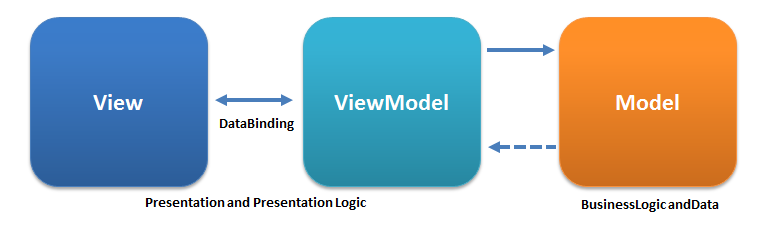
\includegraphics[width=\textwidth]{Figures/WebImages/MVVMPattern}\\
	\caption{The Model View ViewModel Pattern}
	\label{fig:MVVMPattern}
\end{figure}
The \texttt{DriveIT Windows Client} uses the \textit{Model View ViewModel}\footnote{\url{http://en.wikipedia.org/wiki/Model\_View\_ViewModel}} (hereafter \textit{MVVM}) architectural pattern which tries to ensure a clear separation between the \textit{Model} and the \textit{View}. The pattern derives from both the \textit{Model View Controller} pattern and the \textit{Presentation Model} design pattern. Therefore it has some of the same attributes. By using the \textit{MVVM} pattern we created a more testable and easier expandable application.

Furthermore we used \textit{Microsoft Blend}'s\footnote{\url{http://en.wikipedia.org/wiki/Microsoft_Blend}} built in \textit{Actions}\footnote{\url{http://blogs.msdn.com/b/expression/archive/2009/03/23/an-introduction-to-behaviors-triggers-and-actions.aspx}} to encapsulate calls and commands from the \texttt{View} such that \texttt{View} elements would be sent to the \texttt{ViewModel}. These actions are implemented to ensure low coupling.\\

A built-in part of \textit{MVVM} is a version of the \textit{Observer-Pattern}\footnote{\url{http://en.wikipedia.org/wiki/Observer_pattern}}. This is done by creating data-bindings between the \texttt{View} and their \texttt{ViewModel}. In \textit{WPF} this is achieved by having the \texttt{ViewModel}s implement the interface \texttt{INotifyPropertyChanged} which will notify the \texttt{View} when the \texttt{ViewModel} has changed. By using this interface the \texttt{ViewModel} knows nothing of the \texttt{View} and cannot directly change its attributes.

\subsection{Adapter Pattern}
The \textit{Adapter pattern} allows the developer to encapsulate methods and properties of an object in an "Adapter" class. Since the \texttt{DriveIT Windows Client} uses the \textit{MVVM} design pattern, and the \texttt{DriveIT Web API} uses \textit{DTO}s to send and receive data, and \textit{DTO}s are only meant to transfer data, an Adapter Pattern fits perfectly. Almost all single entitiy \texttt{ViewModel}s in the \texttt{DriveIT.WindowsClient.ViewModels} namespace function as adapters for their corresponding \textit{DTO}. E.g the \texttt{CarViewModel} class is an adapter for the \texttt{CarDto} class.\\ 

This implementation provides the \texttt{DriveIT Windows Client} with an easy way to manipulate data, while still retaining the data structure such that entities can be created, read, updated, and deleted over the \texttt{DriveIT Web API} without the having to convert client classes to API classes.

\subsection{Model View Controller Pattern}
\label{sec:MVC}
\begin{figure}[H]
	\centering
	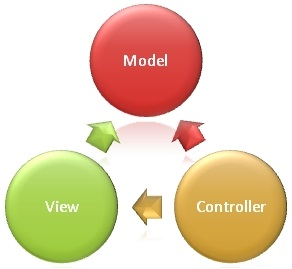
\includegraphics[width=0.5\textwidth]{Figures/WebImages/MVCPattern}\\
	\caption{The Model View Controller Pattern}
	\label{fig:MVCPattern}
\end{figure}
The \texttt{DriveIT Web Client} uses the \textit{Model View Controller}\footnote{\url{http://msdn.microsoft.com/en-us/library/dd381412}} architectural pattern (henceforth \textit{MVC}), which separates the business logic, called \textit{Model}, and the input control, called \textit{Controller}, from the display logic, called \textit{View}.

The \textit{Model} is the part of the application that will be handling the logic for the application data. The \textit{Model}s are being used to store data from the database.
The \textit{View} is the part of the application that will be handling the representation of the data. Mostly this data will be given by the \textit{Model}.
The \textit{Controller} is the part of the application that will be handling the user interaction with the \texttt{DriveIT Web Client}. The \textit{Controller}s read the user input from the \textit{View}s and updates the state of the \textit{Model}.

The \textit{MVC} pattern allows for separation of the \textit{Model}, \textit{View}, and \textit{Controller} classes, such that their individual purposes are clearly distinct from each other. This means that different developers are able to work on each of the individual parts of the \textit{MVC} pattern, e.g we are able to work on the \textit{View} without depending on the business logic or the input.\\

By making this distinction between different parts of the \textit{MVC} pattern, it is easier to test the \texttt{DriveIT Web Client}, and retain a good data structure throughout the development of the \texttt{DriveIT Web Client}.

\subsection{Façade Pattern}
The \textit{Façade design pattern}\footnote{\url{http://en.wikipedia.org/wiki/Facade_pattern}} is used several times in the \texttt{DriveIT System}.
The \texttt{Persistent Storage} subsystem uses a façade pattern to hide the internal subsystems that accomplish the functionality defined in the \texttt{IPersistentStorage} interface.

The \texttt{DriveITContext} in the subsystem is used by the implementer of the \texttt{IPersistentStorage} interface, \texttt{EntityStorage}, but is hidden for users of the interface.

\begin{figure}[H]
	\centering
	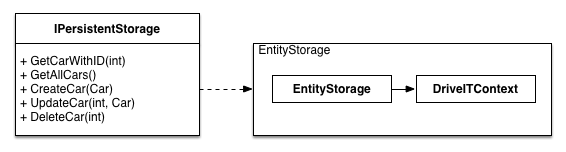
\includegraphics[width=\textwidth]{Figures/FacadePatternPersistentStorage}\\
	% place the figure in the Figures folder (located with the main file)
	% you need to fix the scale a few times to get it right, but latex does not compress so one can always zoom in to see details.
	\caption{The Facade Pattern of IPersistentStorage.}
	\label{fig:The Facade Pattern of IPersistentStorage.}
	% label it something meanfull
\end{figure}

\begin{figure}[H]
	\centering
	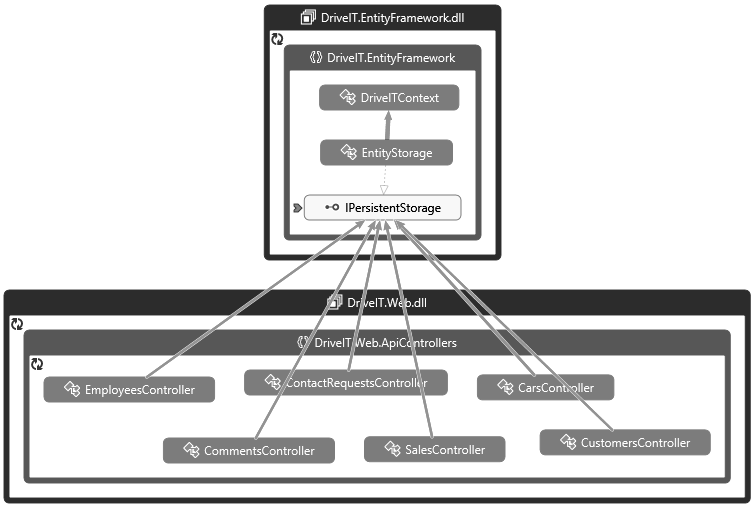
\includegraphics[width=\textwidth]{Figures/FacadeKindOfPattern}\\
	% place the figure in the Figures folder (located with the main file)
	% you need to fix the scale a few times to get it right, but latex does not compress so one can always zoom in to see details.
	\caption{The Facade Pattern Used by the \texttt{DriveIT Web API}.}
	\label{fig:The Facade Pattern Used by the DriveIT Web API.}
	% label it something meanfull
\end{figure}
